\documentclass[12pt]{article}
%\documentclass[envcountsect]{llncs}
\usepackage{fixltx2e} %Use this package and \( \) for best results
\usepackage{amsmath,amssymb,amsthm}
\usepackage{enumitem}
\usepackage{verbatim}
\usepackage{import}
\usepackage[all]{xy}
\usepackage{color}
\usepackage{centernot}
\usepackage{hyperref}

\usepackage{caption,tikz,verbatim,amsmath, amssymb}
\usetikzlibrary{arrows}

%\usepackage{a4wide}
%Theorems & Environments
\newtheorem{theorem}{Theorem}[section]
\newtheorem{lemma}[theorem]{Lemma}
\newtheorem{corollary}[theorem]{Corollary}
\newtheorem{claim}[theorem]{Claim}
\newtheorem{proposition}[theorem]{Proposition}

%\theoremstyle{definition}
\newtheorem{problem}[theorem]{Problem}
\newtheorem{question}[theorem]{Additional questions}
\newtheorem{definition}[theorem]{Definition}
\newtheorem{example}[theorem]{Example}

%\newtheorem{examples}[theorem]{Examples}

%\theoremstyle{remark}
\newtheorem{notation}[theorem]{Notation}
\newtheorem{conclusion}[theorem]{Conclusion}
\newtheorem{remark}[theorem]{Remark}

\setcounter{section}{0}

%Basic Commands
\renewcommand{\implies}{\Rightarrow}
\renewcommand{\iff}{\Leftrightarrow}
\renewcommand{\emptyset}{\varnothing}
%\renewcommand{\epsilon}{\varepsilon}

%Character Commands
\newcommand{\cC}{\mathcal{C}}
\newcommand{\cP}{\mathcal{P}}
\newcommand{\cU}{\mathcal{U}}
\newcommand{\cV}{\mathcal{V}}
\newcommand{\cW}{\mathcal{W}}
\newcommand{\cF}{\mathcal{F}}
\newcommand{\cG}{\mathcal{G}}
\newcommand{\cE}{\mathcal{E}}
\newcommand{\cN}{\mathcal{N}}
\newcommand{\cB}{\mathcal{B}}
\newcommand{\cA}{\mathcal{A}}
\newcommand{\cK}{\mathcal{K}}
\newcommand{\cD}{\mathcal{D}}
\newcommand{\bbR}{\mathbb{R}}
\newcommand{\bbN}{\mathbb{N}}
\newcommand{\bbE}{\mathbb{E}}
\newcommand{\bbQ}{\mathbb{Q}}
\newcommand{\bbZ}{\mathbb{Z}}
\newcommand{\fA}{\mathfrak{A}}
\newcommand{\fB}{\mathfrak{B}}
\newcommand{\fC}{\mathfrak{C}}
\newcommand{\fD}{\mathfrak{D}}

%Math Relations and Operators
\newcommand{\near}{\mathbin{\delta}}	%near
\newcommand{\nnear}{\mathrel{\centernot\delta}}	%not near
\newcommand{\snear}{\mathord{\delta}}	%symbolic near
\newcommand{\nll}{\mathrel{\centernot\ll}}	%not ll
\newcommand{\neare}{\mathrel{\delta_\text{E}}}	%near on End(X)
\newcommand{\nneare}{\mathrel{\centernot{\delta}}_\text{E}}	%not near on End(X)
\newcommand{\sneare}{\mathord{\delta}_\text{E}}
\newcommand{\sll}{\mathord{\ll}}	%symbolic near
\newcommand{\lle}{\mathrel{\ll_\text{E}}}	%ll on End(X)
\newcommand{\slle}{\mathord{\ll_\text{E}}}	%symbolic ll on End(X)
\newcommand{\nell}{\mathrel{\centernot{\ll}}_\text{E}}	%not ll on End(X)
\newcommand{\nearr}[1]{\mathrel{\mathord{\delta}|_#1}}	%Fix spacing issues for a proximity restricted to a subspace
\newcommand{\nnearr}[1]{\mathrel{\mathord{\centernot{\delta}}|_#1}}
\newcommand{\dev}{\ll}
\newcommand{\sdev}{\sll}
\DeclareMathOperator{\obj}{ob}
\DeclareMathOperator{\mor}{M}
\DeclareMathOperator{\End}{End}
\DeclareMathOperator{\RO}{\mathcal{RO}}
\renewcommand{\int}{\operatorname{int}}	%Cannot DeclareMathOperator a defined command
\DeclareMathOperator{\cl}{cl}
\DeclareMathOperator{\Cl}{Cl}
\renewcommand{\a}{\operatorname{a}}
\DeclareMathOperator{\C}{C}
\DeclareMathOperator{\id}{id}
\renewcommand{\o}{\operatorname{o}}
\DeclareMathOperator{\rnd}{rnd}

%Math Text Shortcuts
\newcommand{\textand}{\text{ and }}
\newcommand{\textor}{\text{ or }}
\newcommand{\textst}{\text{ s.t. }}
\newcommand{\textiff}{\text{ iff }}

%Category Commands
\newcommand{\CPTT}{\bf{CPT}_\mathbf{2}}
\newcommand{\DeV}{\bf{DeV}}
\newcommand{\KHaus}{\bf{KHaus}}
\newcommand{\TYCH}{\bf{TYCH}}
\newcommand{\BA}{\bf{BA}}
\newcommand{\ZDCPTT}{\bf{ZDCPT}_\mathbf{2}}
\newcommand{\SET}{\bf{SET}}

\definecolor{darkred}{rgb}{0.3,0.1,0.1}
\definecolor{darkblue}{rgb}{0.1,0.1,0.3}
\definecolor{darkgreen}{rgb}{0.1,0.3,0.1}

\newcommand{\defn}[1]{{\color{darkred}\bf #1}}
\newcommand{\mdefn}[1]{\({\color{darkred}\boldsymbol{#1}}\)}
\newcommand{\respdefn}[2][respectively]{{\color{darkblue}(#1 {\bf #2})}}

\newcommand{\respcolor}{\color{darkblue}}
\newcommand{\resp}[2][respectively]{{\respcolor(#1 #2)}}
\newcommand{\sresp}[1]{\resp[resp.]{#1}}

\newcommand{\prooflabel}[1]{#1:}

\renewcommand{\onecolumn}[1]
{
	\begin{center}
		\makebox{#1}
	\end{center}
}
\renewcommand{\twocolumn}[2]
{
	\begin{center}
		\makebox
		{
			\begin{minipage}[b]{0.5\linewidth}#1\end{minipage}
			\hspace{0.3cm}
			\begin{minipage}[b]{0.5\linewidth}#2\end{minipage}
		}
	\end{center}
}
\newcommand{\threecolumn}[3]
{
	\begin{center}
		\makebox
		{
			\begin{minipage}[b]{0.33\linewidth}#1\end{minipage}
			\hspace{0.3cm}
			\begin{minipage}[b]{0.33\linewidth}#2\end{minipage}
			\hspace{0.3cm}
			\begin{minipage}[b]{0.33\linewidth}#3\end{minipage}
		}
	\end{center}
}
\title{{\small \bf Google Summer of Code 2015}\\Extending PLN to Auto-Epistemic Reasoning }
\author{Sumit Sourabh \\ \small{Institute for Logic, Language and Computation}, \\ {\small University of Amsterdam, The Netherlands.} \\\\ Mentor: Matthew Ikle \\ \small{Adams State University, USA.} }
\date{}
\begin{document}
\maketitle
\begin{abstract}
We extend the Probabilistic Logic Network (PLN) framework by developing an auto-epistemic theory for PLN. We list rules for inference for epistemic reasoning using both simple and complex truth values. We also add rules for inference for belief revision based on Jeffrey's rule. 
\end{abstract}

\section{Belief Predicates}

{\em  Probabilistic Logic Network} (PLN) \cite{PLN} is a framework for probabilistic inference. It uses probabilistic inference rules similar to the ones used in term logic to calculate the probabilistic truth value at a conclusion, based on the probabilistic truth values at the premise. 


 %Modal logics are the best known logics other than classical logic. In their modern form they are enriched formal languages in which one can express and reason about \emph{modes of truth}, e.g., the {\em possible}, {\em necessary}, {\em usual} or {\em past} truth of propositions. Syntactically, the language of modal logic is an expansion of classical propositional logic with new connectives, so as to have formulas such as $\Box \phi$ or $\Diamond\phi$, the intended meaning of which respectively is `$\varphi$ is necessary/obligatory/always true in the past$\dots$' and `$\varphi$ is possible/permitted/sometimes true in the past$\dots$'. Modal logics are widely applied in fields as diverse as program verification in theoretical computer science \cite{GrVe08}, natural language semantics \cite{vBM1997}, multi-agent systems in AI \cite{Gabbay:1993}, %\marginpar{\raggedright\tiny{{\em Johan F.A.K. van Benthem on Logical and Informational Dynamics}, Springer series {\em Outstanding Contributions to Logic}, edited by A. Baltag and S. Smets, Springer, in print 2014.}}, foundations of arithmetics \cite{ArtBek05}, game theory in economics \cite{ParPau03}, categorization theory in social and management science \cite{PoHa10}.


Epistemic logic (\cite{Hoekverbrugge,Kooi07}) is an important subfield of modal logic (\cite{BRV,CZ97}) which studies \emph{Knowledge} and \emph{Belief} as  modalities. In particular, for an agent $i$, $K_i\varphi$ denotes that the agent $i$ knows $\varphi$ and $B_i \varphi$ denotes that the agent $i$ believes $\varphi$. The study of beliefs plays an important role in the multi-agent world, since in order to act, an agent  needs to reason about what other agents believe. Epistemic logic has many applications \cite{Meyer} in computer science and economics, and in particular in robotics, network security and cryptography applications to the study of social and coalition interactions. %The formulas are interpreted in a \emph{frame} $(W,R)$ where $W$ is a non-empty set of states and $R$ is a binary relation on $W$. 



An interesting and useful extension of PLN would be to incorporate epistemic logic into its framework. At present, PLN has rules for temporal reasoning which uses probabilistic predicates such as \texttt{hold (event)}, \texttt{initiate (event)} and \texttt{terminate(event)}. In the same spirit, we can introduce the following probabilistic predicates for epistemic reasoning:

\begin{itemize}
\item
\texttt{believe$_i$ (term) <truth value> <confidence>= ``the degree of belief of the agent $i$ in term is greater than or equal to the truth value with a certain confidence value.''}
\item

\texttt{believeAt$_i$ (term) [L,U] <confidence> = ``the agent $i$ believes the term is true with a truth value which lies in the interval [L,U] with a certain confidence.''} 

%\item

%\texttt{believeAtState$_i$ (term, setofstates) <truth value> = ``there is a state s in the set setofstates such that\\  believesAt$_i$ (proposition,s) with a certain truth value.}"


\end{itemize}
%The above predicates are maps from propositions to probabilistic truth values. For instance, the predicate \texttt{believe (proposition)} will take a proposition as an input and produce a probabilistic truth value which is the degree of belief of an agent in that proposition.
 
\section{Epistemic reasoning} 

In this section we provide inference rules to compute the truth values of complex terms involving belief predicates. For simplicity, we focus on the belief predicate \texttt{believe$_i$ (term) <truth value>}. Before we list the inference rules, we first mention our semantic environment. 

\paragraph{Semantics.} Our semantic environment consists of a probabilistic model $(W,P,v)$, where 
\begin{enumerate}
\item
$W$ is a non-empty finite set of ``possible worlds'' or states.
\item
$P$ is a map which maps every possible world $w$ to a probability space $(W,\mathcal{P}(W),\mu_{w})$, where $\mu_{w}: \mathcal{P}(W)\to[0,1]$ is a probability measure, that is, it satisfies the following conditions:

\begin{enumerate}
\item
$0\leq \mu_{w}(X)\leq 1$, for all $X\in \mathcal{P}(W)$.
\item
$\mu_{w}(\emptyset)=0$ and $\mu_{w}(W)=1$.
\item
If $X,Y\in \mathcal{P}(W)$ are disjoint sets, then $\mu_{w}(X\cup Y)=\mu_{w}(X)\cup\mu_{w}(Y)$. 
\end{enumerate}
\item
$v$ is an assignment which provides truth assignments to primitive terms. 
\end{enumerate}
The semantics of the belief predicate is given as follows. For an agent $i$ , the term \texttt{believe$_i$ A <s>} denotes that the agent believes in the term \texttt{A} with truth value which is \emph{greater than or equal to} \texttt{<s>}. This term is true at a possible world $w$ in our model $\mathcal{M} = (W,P,v)$ iff $\mu_{w}(v(\texttt{A}))\geq s$, where $v(\texttt{A})$ is the set of worlds where the term \texttt{A} is true. The term \texttt{believe$_i$ A <s>} is true in the model if it is true at every possible world of the model. 





\begin{example}{\em We illustrate our semantics using an example. Let there be two fair coins $C_1$ and $C_2$. We model an agent's beliefs about the possible outcomes of the two coins. Let $H_1$ and $H_2$ be primitive terms which denote that the outcomes of coins $C_1$ and $C_2$ are heads. Consequently, the terms $\mbox{\texttt{NOT}} H_1$ and $\mbox{\texttt{NOT}} H_2$ denote that the outcome of the coins are tails. 

\begin{figure}
\begin{center}
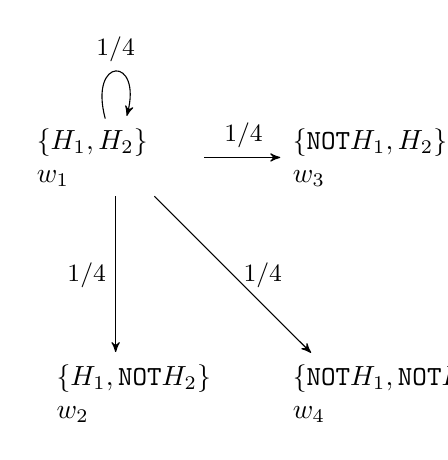
\begin{tikzpicture}[->,>=stealth',shorten >=1pt,auto,node distance=3cm,main node/.style={}]

  \node[text width=2cm] (1) {$\{H_1,H_2\}$ \\$w_1$};
  \node[text width=1.5cm] (2) [below of=1] {$\{H_1, \mbox{\texttt{NOT}} H_2$\}\\$w_2$};
  \node[text width=1.5cm] (3) [right of=1] {$\{\mbox{\texttt{NOT}} H_1, H_2\}$ \\$w_3$};
  \node[text width=1.5cm] (4) [below of=3] {$\{\mbox{\texttt{NOT}} H_1,\mbox{\texttt{NOT}} H_2\}$\\$w_4$};
  \path[every node/.style={font=\small}]
  (1) edge [loop above] node [above] {1/4} (1)
    edge node [above] {1/4} (3)
   edge node [right] {1/4} (4)
   edge node [left] {1/4} (2)
   ;
 
\end{tikzpicture}
\caption{Possible worlds and probabilities $P_1$ for unbiased coins}
\label{fig:possiblew}
\end{center}
\end{figure}

The possible worlds for the agent are $w_1$, $w_2$, $w_3$ and $w_4$ as denoted in Figure \ref{fig:possiblew}. The probability assignments are $P_1$, $P_2$, $P_3$ and $P_4$ which map the possible worlds to probability measures $\mu_{w_1},\mu_{w_2},\mu_{w_3}$ and $\mu_{w_4}$, respectively, and which are defined as follows:\\

\begin{center}
\begin{tabular}{|c|c|c|c|c|}
\hline
&  $\{w_1\}$ &$\{w_2\}$ &$\{w_3\}$ & $\{w_4\}$\\ 
\hline
$\mu_{w_1}$& 1/4 & 1/4 & 1/4 &1/4\\ 
\hline
$\mu_{w_2}$& 1/4 & 1/4 & 1/4 &1/4\\ 
\hline
$\mu_{w_3}$& 1/4 & 1/4 & 1/4 &1/4\\ 
\hline
$\mu_{w_4}$& 1/4 & 1/4 & 1/4 &1/4\\ 
\hline
\end{tabular}
\end{center}

In Figure \ref{fig:possiblew}, the probability maps can be thought of as probabilistic transitions from a certain state to other states in the model. According to this perspective, our model is similar to a relational structure, which is used in modal logic to interpret the semantics of modal formulas.

Since the agent knows that both the coins are unbiased, each of the four possible worlds have equal probability. In any possible world, the agent believes that each possible world can occur with a probability of 1/4. Figure \ref{fig:possiblew} represents the probability measure $\mu_{w_1}$. In the above model the degree of belief of agent in the term $H_1$ is at least 1/2. In other words the term \texttt{believe$_i$ $H_1$ <1/2>} is true in any state of the model. To see this, let us evaluate the term at the state $w_1$. The term $H_1$ is true at $w_1$ and $w_2$. Hence, the degree of belief of the agent in the term $H_1$ at $w_1$ is the value of $\mu_{w_1} (\{w_1,w_2\})$. Since $\mu_{w}$ is a probability measure, $\mu_{w_1} (\{w_1,w_2\})=\mu_{w_1}\{w_1\}+\mu_{w_1}\{w_2\} =1/4 + 1/4 =1/2$. Hence, the degree of belief of the agent in the term $H_1$ is greater than or equal to 1/2.      

}
\end{example}

\begin{example} {\em We consider a different situation where the agent knows that the first coin $C_1$ is biased in such a way that the probability of heads is 2/3  and that of tails is 1/3, and the second coin $C_2$ is unbiased. The probability measure for individual states changes to the following values.

\begin{center}
\begin{tabular}{|c|c|c|c|c|}
\hline
&  $\{w_1\}$ &$\{w_2\}$ &$\{w_3\}$ & $\{w_4\}$\\ 
\hline
$\mu_{w_1}$& 1/3 & 1/3 & 1/6 &1/6\\ 
\hline
$\mu_{w_2}$& 1/3 & 1/3 & 1/6 &1/6\\ 
\hline
$\mu_{w_3}$& 1/3 & 1/3 & 1/6 &1/6\\ 
\hline
$\mu_{w_4}$& 1/3 & 1/3 & 1/6 &1/6\\ 
\hline
\end{tabular}
\end{center}


The possible worlds and the transition probabilities are expressed in Figure \ref{fig:possiblewu}. The probability values in the above table can be explained as follows. Since the agent knows that the first coin is biased, so the probability of the world $w_1$ is probability of occurrence of heads for the unbiased coin, times the probability of occurrence of the heads of the unbiased coin. Therefore, $\mu_1\{w_1\}=2/3\times 1/2 =1/3$. Similarly, $\mu_1\{w_3\}=1/3\times 1/2 =1/6$. 

In this model, the term \texttt{believe$_i$ $H_1$ <2/3>} is true. This is because the $H_1$ is true in the worlds $w_1$ and $w_2$. Hence, the degree of belief of the agent at world $w_1$ is given by $\mu_{w_1}(\{w_1,w_2\})=\mu_{w_1}\{w_1\}+\mu_{w_1}\{w_2\} =1/3 + 1/3 =2/3$. This degree of belief of the agent in term $H_1$ is greater than the previous example, since in this case, the agent knows that the first coin is biased towards head occurring with a higher probability.
\begin{figure}
\begin{center}
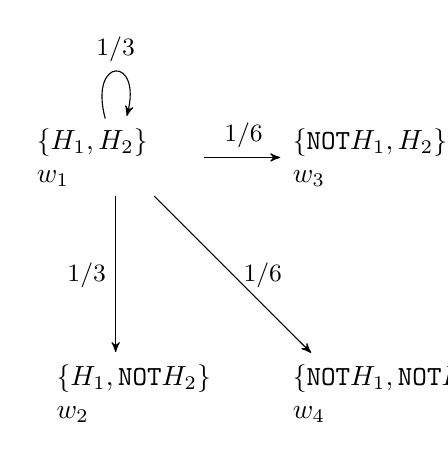
\begin{tikzpicture}[->,>=stealth',shorten >=1pt,auto,node distance=3cm,main node/.style={}]

  \node[text width=2cm] (1) {$\{H_1,H_2\}$ \\$w_1$};
  \node[text width=1.5cm] (2) [below of=1] {$\{H_1, \mbox{\texttt{NOT}} H_2$\}\\$w_2$};
  \node[text width=1.5cm] (3) [right of=1] {$\{\mbox{\texttt{NOT}} H_1, H_2\}$ \\$w_3$};
  \node[text width=1.5cm] (4) [below of=3] {$\{\mbox{\texttt{NOT}} H_1,\mbox{\texttt{NOT}} H_2\}$\\$w_4$};
  \path[every node/.style={font=\small}]
  (1) edge [loop above] node [above] {1/3} (1)
    edge node [above] {1/6} (3)
   edge node [right] {1/6} (4)
   edge node [left] {1/3} (2)
   ;
 
\end{tikzpicture}
\caption{Possible worlds and probabilities for biased coins}
\label{fig:possiblewu}
\end{center}
\end{figure}}

\end{example}

\begin{example}{\em We consider a third case when there is a single coin, and the agent does not know whether the coin is fair or biased (say, towards heads). His belief in the coin being fair is higher than the coin being biased towards heads. In this case the possible worlds are:
\begin{itemize}
\item $w_1$: The outcome of the coin is a head and it is a fair coin.
\item $w_2$: The outcome of the coin is a tail and it is a fair coin.
\item $w_3$: The outcome of the coin is a head and it is a biased coin.
\item $w_4$: The outcome of the coin is a tail and it is a biased coin.

\end{itemize}

Suppose the agent believes with a high probability of 9/10 that the coin is fair, and his belief that the coin is biased is 1/10. Suppose the probability of heads in the biased coin is 2/3. The probabilities distributions for the possible worlds which model this context are as follows: 
\begin{center}
\begin{tabular}{|c|c|c|c|c|}
\hline
&  $\{w_1\}$ &$\{w_2\}$ &$\{w_3\}$ & $\{w_4\}$\\ 
\hline
$\mu_{w_1}$& 0.465 & 0.435 & 0.051 & 0.048\\ 
\hline
$\mu_{w_2}$& 0.465 & 0.435 & 0.051 & 0.048\\ 
\hline
$\mu_{w_3}$& 0.465 & 0.435 & 0.051 & 0.048\\ 
\hline
$\mu_{w_4}$& 0.465 & 0.435 & 0.051 & 0.048\\ 
\hline
\end{tabular}
\end{center}
\begin{figure}
\begin{center}
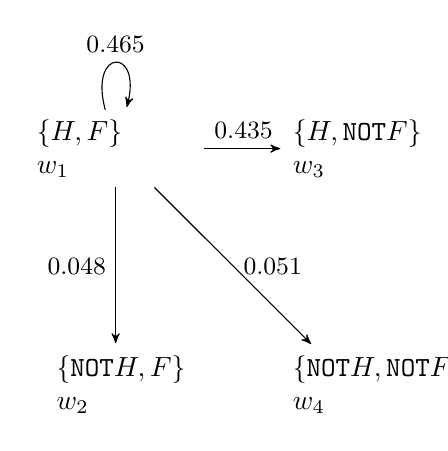
\begin{tikzpicture}[->,>=stealth',shorten >=1pt,auto,node distance=3cm,main node/.style={}]

  \node[text width=2cm] (1) {$\{H,F\}$ \\$w_1$};
  \node[text width=1.5cm] (2) [below of=1] {$\{\mbox{\texttt{NOT}} H, F$\}\\$w_2$};
  \node[text width=1.5cm] (3) [right of=1] {$ \{H, \mbox{\texttt{NOT}} F\}$ \\$w_3$};
  \node[text width=1.5cm] (4) [below of=3] {$\{\mbox{\texttt{NOT}} H,\mbox{\texttt{NOT}} F\}$\\$w_4$};
  \path[every node/.style={font=\small}]
  (1) edge [loop above] node [above] {0.465} (1)
    edge node [above] {0.435} (3)
   edge node [right] {0.051} (4)
   edge node [left] {0.048} (2)
   ;
 
\end{tikzpicture}
\caption{Possible worlds and probabilities for a single coin}
\label{fig:possiblewusc}
\end{center}
\end{figure}

To illustrate how the transition probabilities in the table are calculated, we compute it for the the world $w_1$. The total probability of a head is equal to the sum of the probability of the head on the condition that the coin is fair, and the probability of the head on the condition that the coin is biased. Therefore, $P(H) = P(H|F)*P(F) + P(H| NOT F)*P(NOT F)$, which is equal to $1/2*9/10 + 2/3*1/10$. So the transition probability at the world $w_1$ is the product of the probability of the head as an outcome times the probability of the coin being fair which comes out to be $0.465$. The other transition probabilities are computed similarly. }
\end{example}

\subsection{Simple inference rules using simple truth values}
Suppose an agent $i$ believes a term \texttt{A} with a truth value of at least $s$ and a confidence $c$. As mentioned earlier, using the PLN style terminology, this can be expressed as: \texttt{believe$_i$ A <$s$> <$c$>}. The inference rules for the belief predicates are listed below.

\begin{itemize}
\item
\noindent The inference rule for the epistemic negation \texttt{ENOT} is:  

\noindent \texttt{believe$_i$ (A) <$s*(1-\epsilon)$> <$c_1$>} \\
 $\vdash$
\texttt{believe$_i$ (ENOT A) <$\epsilon$> <$c_2$>} \\

\noindent where, $\epsilon>0$ is small positive constant and $c_2 >c_1$ . Intuitively, it means that if an agent believes a term with a truth value of at least $s*(1-\epsilon)$, then he believes the negation of that term with a truth value of at least $\epsilon$. Since the truth value interval of the inference increases, the confidence of the agent in that truth value also increases from $c_1$ to $c_2$. 

\item  \noindent The inference rule for the epistemic conjunction \texttt{EAND} is: 

\noindent \texttt{believe$_i$ (A) <$s_1$> <$c_1$>}\\
 \texttt{believe$_i$ (B) <$s_2$> <$c_2$>}\\
 $\vdash$
\texttt{believe$_i$ (A EAND B) <t> <$c$>}  

where, $t = \mathsf{max}(s_1+s_2-1,0)$, and $c=\mathsf{min}(c_1,c_2)$. Intuitively, this means that if an agent $i$ believes that term \texttt{A} is true with a probability $s_1$ and term \texttt{B} is true with a probability $s_2$, then he believes terms \texttt{A} and \texttt{B} together to be true with a probability $\mathsf{max}(s_1+s_2-1,0)$.



 \item \noindent The inference rule for the epistemic disjunction \texttt{EOR} is: 

\noindent \texttt{believe$_i$ (A) <$s_1$> <$c_1$>}\\
 \texttt{believe$_i$ (B) <$s_2$> <$c_2$>}\\
 $\vdash$
\texttt{believe$_i$ (A EOR B) <t> <$c$>}

where $t = \mathsf{min}(s+t,1)$, and $c=\mathsf{min}(c_1,c_2)$. The soundness of this inference rule follows from the inference rules for \texttt{ENOT} and \texttt{EAND}.

 
\end{itemize}

\paragraph{Soundness of simple inference rules.} Consider the epistemic negation rule. We will show that this rule is sound at an arbitrary world $w_1$ of our probabilistic model $(W,P,v)$.  Suppose the term $\texttt{A}$ is true in the set $X\subseteq W$ of possible worlds. Then its negation is true in the set $W\setminus X$. Since the degree of belief in \texttt{A} is \texttt{<$s*(1-\epsilon)$>}, which means $\mu_{w_1}(X) \geq s*(1-\epsilon)$. Moreover, $\mu_{w_1}$ is a probability measure. So, $\mu_{w_1}(X) +\mu_{w_1} (W\setminus X) = 1$. Therefore, $\mu_{w_1} (W\setminus X)\geq \epsilon$.  This justifies our rule for the epistemic negation. 



Next, we consider the epistemic conjunction rule. Suppose \texttt{believe$_i$ (A) <$s_1$>} and \texttt{believe$_i$ (B) <$s_2$>} are true in our probabilistic model $(W,P,v)$ at an arbitrary world $w_1$. Let $X\subseteq W$, $Y\subseteq W$ be the set of possible worlds where the terms \texttt{A} and \texttt{B} are true, respectively. This implies that $\mu_{w_1} (X) \geq s_1$ and $\mu_{w_1} (Y) \geq s_2$. The set of possible worlds where both \texttt{A} and \texttt{B} are true is the intersection of $X$ and $Y$, that is, $X\cap Y$. Since $\mu_{w_1}$ is a probability measure, $\mu_{w_1} (X\cap Y) =\mu_{w_1}(X) + \mu_{w_1}(Y) -\mu_{w_1}(X\cup Y)$. Therefore, $$\mu_{w_1} (X\cap Y)\geq \mu_{w_1}(X) + \mu_{w_1}(Y)-1,$$ 
since, $\mu_{w_1}(X\cup Y)\leq 1.$ This justifies our inference rule for epistemic conjunction.


Finally, consider the epistemic disjunction rule. % From basic probability theory, we know that if $\mu$ is a probability measure, then for $X,Y\subseteq W$$$ \mu (X\cap Y) + \mu(X\cup Y) =\mu (X) +\mu (Y).$$ 
Suppose \texttt{believe$_i$ (A) <$s_1$>} and \texttt{believe$_i$ (B) <$s_2$>} are true in our probabilistic model $(W,P,v)$ at an arbitrary world $w_1$. Since $\mu$ is a probability measure,  $\mu_{w_1} (X\cup Y) =\mu_{w_1}(X) + \mu_{w_1}(Y) -\mu_{w_1}(X\cap Y)$. From the epistemic conjunction rule, we know that $\mu_{w_1}(X\cap Y)\geq \mathsf{max}(s_1+s_2 -1,0)$. Therefore, a simple calculation shows that $\mu_{w_1} (X\cup Y) \geq \mathsf{min}(s_1+s_2,1)$. Hence, our inference rule for the epistemic disjunction is sound. 


\subsection{Complex inference rules using simple truth values} 
Other complex inference rules for the epistemic predicate  \texttt{believe$_i$ (term) <truth value>} can be summarized as follows.

\begin{enumerate}
\item
\texttt{(A) <$s$> <$c$>}\\
$\vdash$
\texttt{believe$_i$ (A) <$s*(1-\epsilon)$> <$c$>}

where, $\epsilon$ is a small positive constant tending to 0. The above inference rule means that if a term is true with a degree $s$, then the agent believes it with a truth value $s*(1-\epsilon)$. The $\epsilon$ is the factor which accounts for the dynamic nature of the environment.
\item
\texttt{believe$_i$ A <$s_1$> <$c_1$>}\\
$\vdash$
\texttt{believe$_i$ A <$s_2$> <$c_2$>}

where, $0\leq s_2\leq s_1\leq 1$ and $c_2>c_1$. The above inference rule means that if an agent believes a term \texttt{A} with a truth value $s_1$, then he also believes the same term \texttt{A} with any lower truth value $s_2\leq s_1$. An important remark is that the confidence value of the agent's belief in a lower truth value increases because the interval of the belief now increases to $[s_1,1]$ to $[s_2,1]$  
\item
\texttt{Implication (A) (B) <$s$> <$c$>}\\
$\vdash$
\texttt{Implication (believe$_i$ A <t>) (believe$_i$ B <t>) <$s*(1-\epsilon)$> <$c$>}

where \texttt{Implication} is the PLN implication relation. The above inference intuitively means that if the term \texttt{A} implies the term \texttt{B}, then the belief of the agent in the term \texttt{A} with a truth value $t$ implies that the agent believes in the term $B$ with the same truth value. 



\item
\texttt{Equivalence (A) (B) <$s$> <$c$>}\\
$\vdash$
\texttt{Equivalence (believe$_i$ (A) <t>)}\texttt{(believe$_i$ (B) <t>) <$s*(1-\epsilon)$> <$c$>}

The above inference rule intuitively means that if two terms \texttt{A} and \texttt{B} are equivalent, and an agent believes the term \texttt{A} with a truth value $s$, then he also believes the term \texttt{B} with a truth value $s$.

\item
\texttt{believe$_i$ A <$s$>  <$c_1$> }\\
$\vdash$
\texttt{believe$_i$  (believe$_i$ A) <0.95> <$c_2$>}

where, $c_2 < c_1$. The above inference rule means that if an agent believes a term \texttt{A} with a truth value \texttt{<s>}, then he his belief about his belief about the proposition \texttt{A} has a truth value of 1. In other words, an agent trusts his own belief. It is important to note that the confidence of the agent decreases as the truth value interval increases.

\end{enumerate}

\paragraph{Soundness of complex inference rules.} We show that each of the above complex rules are sound with respect to a probabilistic model $(W,P,v)$. We assume, without loss of generality, that we are evaluating the terms at an arbitrary world $w\in W$ of the model.\\

 1. Since the truth value of term \texttt{A} is 1, the set of worlds where $A$ is true is $W$, that is, at all worlds in the model. Hence, the degree of belief in the term \texttt{A} at the world $w$ is $\mu_{w} (W) =1$, since $\mu_w$ is a probability measure.\\

2. Since \texttt{Implication (A) (B)} holds, the set of worlds where \texttt{A} is true is a subset of the set of worlds where \texttt{B} is true. Let $X,Y\subseteq$ respectively be the sets of worlds where terms $A$ and $B$ are true. Then $X\subseteq Y$. Therefore, since $\mu$ is a probability measure, $\mu(X)\subseteq \mu (Y)$ which implies \texttt{Implication (believe$_i$ A <s>) (believe$_i$ B <s>)}.\\

3. Since the term \texttt{believe$_i$ A <$s_1$> } is true in the model, we have $\mu_w(X)\geq s_1$, where $X$ is the set of worlds where the term \texttt{A} is true. But $\mu_w(X)\geq s_1$ implies $\mu_w(X)\geq s_2$ for any $0\leq s_2\leq s_1$. Hence, \texttt{believe$_i$ A <$s_2$> } is true in our model. \\

4. Since terms \texttt{A} and \texttt{B} are equivalent, the set of possible worlds in the model where the term \texttt{A} is true (let it be $X\subseteq W$) is same as the set of possible worlds where the term \texttt{B} is true. Moreover, from \texttt{(believe$_i$ (A) <s>)}, we have $\mu_w(X)\geq s$, which implies \texttt{(believe$_i$ (B) <s>)}.\\
 
5. Since \texttt{believe$_i$ A <s>} is true at every state in the model, we have $v(\texttt{believe$_i$ A <s>})=W$. Hence, \texttt{believe$_i$  (believe$_i$ A) <1>} is true, as $\mu_w(W)=1.$



%\paragraph{Computing probabilistic truth values.} We now define inference rules for these predicates.  The truth values of the inference rules can be calculated by relying on the laws of probability, which is normally the case for other PLN inference rules. 



%In order to compute the truth values of predicates, we can use the sampling algorithm proposed in the following paper.

% A. Shirazi and E. Amir. Probabilistic modal logic. In \emph{Proc. of the 22nd National Conference on Artificial Intelligence (AAAI)}, 2007.

 %Informally, the algorithm calculates the probabilistic truth values of formulas on probabilistic frames. The number of states in which the formula $x$ is true has a binomial distribution. In order to compute the truth value of a formula at a particular state, $M$ states are sampled from that distribution. This is then used to construct a \emph{sampled expression tree}, using which the probability values are estimated.

\subsection{Belief revision using simple truth values} In the real world, an agent may revise his or her own belief after receiving new (trusted) information. For instance, an agent's belief that all american presidents are white will be revised after receving the information that Obama has been elected a president. The information can be certain (if it comes from a trusted source) as well as uncertain (if the source is not trustworthy. We would like to add belief predicates which also model such updates in the the probabilistic truth values. Examples of such predicates are the following:

\begin{itemize}
\item
\texttt{believe (proposition, certaininformation) = ``the agent \\ believes in the proposition after becoming aware of the\\ certain information with a certain truth value''}

\item
\texttt{believe (proposition, uncertaininformation, p) = ``the agent believes in the proposition after becoming aware of the \\ uncertain information with a degree of uncertainty p (where, $0\leq p\leq 1) $ with a certain truth value''}

\end{itemize}


\paragraph{Jeffery's rule.} Suppose the initial situation is that the agent believes in a proposition $A$ with a truth value \texttt{<$s$>}. Since the context of the agent is dynamic, he revises his beliefs in accordance with the new information which he receives. We assume that the new information $Inf$ tells the agent that mutually exclusive propositions $B_1, B_2, \ldots, B_n$ hold with truth values $a_1,\ldots,a_n$ such that $a_1+\ldots+a_n=1$. Then, the agent revises the truth value of his belief in the proposition $A$ to the value $a_1 Pr(A|B_1) + \ldots + Pr(A|B_n)$.

\paragraph{Inference rule for belief revision.} We adapt the Jeffery's rule \cite{Jeffrey1983} to the context of PLN truth values as follows.\\

\noindent \texttt{believe$_i$ A <$s$>}\\
\noindent \texttt{Inf <$t$>}\\
$\vdash$
\noindent \texttt{believe$_i$ A <$u$>}\\

where, $u=t*(a_1 Pr(A|B_1) + \ldots + Pr(A|B_n))$. Intuitively, this rule states that of the agent believes in a proposition \texttt{A} with a truth value of $s$, and he receives information \texttt{Inf} which has a truth value of $t$, he will update or revise his belief in \texttt{A} according to the Jeffery's rule as mentioned above. 

\begin{example}{\em We illustrate the above inference rule by means of an example. Consider one of the earlier examples where the agent is not sure whether the coin is biased or not. Recall that his belief that the outcome is a head is equal to $1/2*9/10 + 2/3*1/10$, since he believed that the probability of the coin being biased is $1/10$.

 Now his friend informs him that the coin is biased with a high probability of 5/6 . Since this friend does not always speak the truth, the agent's belief in his friend's claim is 3/4. Using Jeffery's rule, the new belief of the agent in the outcome being a head is $u= t* (a_1*Pr(H|F)+a_2*P(H| NOT F)) = 3/4 * (1/2*1/6 + 2/3*5/6) $.
}
\end{example}

\section{Indefinite Truth Values} In this section we introduce inference rules for belief predicates using  indefinite truth values. In PLN \emph{indefinite probabilities} provide an alternative technique to quantify  uncertainty. An indefinite probability is quadruple $<[L,U],b,k>$, where $[L,U]$ is the probability interval,  $b$ is the  credibility level, and $k$ is the lookahead parameter. The intuitive semantics of the indefinite probability is that after $k$ more observations the conclusion of the inference will be in the interval $[L,U]$ with a probability $b$. For inference rules, the indefinite probabilities are computed as follows.

\begin{enumerate}
\item
Let $[L_i, U_i]$ be the interval premise probabilities. In order to compute indefinite probabilities of the conclusion, we find a distribution $[L1_i,U1_i]\supset [L_i,U_i]$ such that these have $[L_i,U_i]$ as $(100.b_i)\%$ credible intervals.
\item
In the second step, for each premise $n_1$ values are randomly selected from the distribution found in the first step. These $n_1$ values provide the values for the means for our first-order distributions. For each of our $n_1$ first-order distributions, $n_2$ values are selected to represent the first-order distribution. The applicable inference rule are applied  to each of the $n_2$ values for each first-order distribution to generate the final distribution of first-order distributions of probabilities.
\item
 Finally, we calculate the mean of each distribution and then find a $(100.b\%)$ credible interval, $[L_f,U_f]$, for this distribution of means.

\end{enumerate}



\subsection{Simple inference rules} In order to extend the inference rules for epistemic reasoning to indefinite truth values, we propose the following. Suppose an agent $i$ believes that a term \texttt{A} has a truth value which lies in the interval $[L,U]$ with a confidence level $b$. In the PLN style terminology, using indefinite truth values this can be expressed as: \texttt{believe$_i$ A $[L,U]$ <$b$>}. The inference rules for the belief predicates are listed below.

\begin{itemize}
\item
\noindent The inference rule for the epistemic negation \texttt{ENOT} using an indefinite truth value is:  

\noindent \texttt{believe$_i$ (A) $[L_1,U_1]$ <$b$>} \\
 $\vdash$
\texttt{believe$_i$ (ENOT A) $[L,U]$ <$b$>} \\

\noindent where, $\epsilon>0$ is small positive constant. The interval $[L,U]$ in the conclusion can be computed using the heuristic that \texttt{believe$_i$ (NOT A)} =  1- \texttt{belief}$_i$ (A).

\item  \noindent The inference rule for the epistemic conjunction \texttt{EAND} using an indefinite truth value is: 

\noindent \texttt{believe$_i$ (A) $[L_1,U_1]$ <$b$>} \\
 \texttt{believe$_i$ (B) $[L_2,U_2]$ <$b$>}\\
 $\vdash$
\texttt{believe$_i$ (A EAND B) $[L,U]$ <$b$>} 

where, the interval $[L,U]$ can be computed using the heuristic that \texttt{believe$_i$ (A EAND B)} =  $\mathsf{max}$ (\texttt{belief}$_i$ (A) + \texttt{belief}$_i$ (B) -1, 0).



 \item \noindent The inference rule for the epistemic disjunction \texttt{EOR} is: 

\noindent \texttt{believe$_i$ (A) $[L_1,U_1]$ <$b$>} \\
 \texttt{believe$_i$ (B) $[L_2,U_2]$ <$b$>}\\
 $\vdash$
\texttt{believe$_i$ (A EOR B) $[L,U]$ <$b$>} 

where, the interval $[L,U]$ can be computed using the heuristic that \texttt{believe$_i$ (A OR B)} =  $\mathsf{min}$ (\texttt{belief}$_i$ (A) + \texttt{belief}$_i$ (B), 1).
\end{itemize}


\subsection{Complex inference rules} 
Other complex inference rules for the epistemic predicate  \texttt{believe$_i$ (term) <truth value>} using the indefinite probabilities can be summarized as follows.

\begin{enumerate}
%\item
%\texttt{(A) $[L_1,U_1]$ <$b$>}\\
%$\vdash$
%\texttt{believe$_i$ (A) $[L_1,U_1]$ <$b$>}

%The above inference rule means that if a term is true with a degree $s$, then the agent believes it with a truth value $s*(1-\epsilon)$. The $\epsilon$ is the factor which accounts for the dynamic nature of the environment.
\item
\texttt{believe$_i$ A $[L_1,U_1]$ <$b$>}\\
$\vdash$
\texttt{believe$_i$ A $[L,U]$ <$b$>}

where, $[L,U]\subseteq [L_1,U_1]$. The above inference rule means that if an agent believes that the truth value of a term \texttt{A} lies in the interval $[L_1,U_1]$ with a confidence level $b$, then he believes that the truth value of the term \texttt{A} lies in in the interval $[L,U]$, where $[L,U]\subseteq [L_1,U_1]$. \\
\item
\texttt{believe$_i$ (A) $[L_1,U_1]$ <$b$>}\\
\texttt{Implication (A) (B) $[L_2,U_2]$ <$b$>}\\
$\vdash$
\texttt{believe$_i$ (B) $[L,U]$ <$b$>) }

where \texttt{Implication} is the PLN implication relation. The above inference intuitively means that if the term \texttt{A} implies the term \texttt{B} with a certain indefinite probability $[L_2,U_2]$, and the truth value of the agent in term \texttt{A} lies in the interval $[L_1,U_1]$, then the agent believes in the term $B$ with the truth vale lying in the interval $[L,U]$. The interval $[L,U]$ can be calculated using the heuristic that the belief of the agent in term \texttt{B} lies in the interval [\texttt{belief$_i$ A AND B, $1-$ (belief$_i$ A -belief$_i$ A AND B)}] = [$\mathsf{max}$ (\texttt{belief}$_i$ (A) + \texttt{belief}$_i$ (B) -1, 0), 1 - (belief$_i$ A - $\mathsf{max}$ (\texttt{belief}$_i$ (A) + \texttt{belief}$_i$ (B) -1, 0)) ].   \\

%\item
%\texttt{Implication (A) (B) $[L,U]$ <$b$>}\\
%$\vdash$
%\texttt{Implication (believe$_i$ A $[L_1,U_1]$ <$b$>) (believe$_i$ B $[L_1,U_1]$ <$b$>) $[L,U]$ <$b$> }

%where \texttt{Implication} is the PLN implication relation. The above inference intuitively means that if the term \texttt{A} implies the term \texttt{B} with a certain indefinite probability, then the belief of the agent in the term \texttt{A} with a truth value in the interval $[L_1,U_1]$ implies that the agent believes in the term $B$ with the truth vale lying in the same interval. \\


\item
\texttt{Implication} (A) (B) $[L_1,U_1]$ <$b$>\\
\texttt{Implication} (B) (A) $[L_2,U_2]$ <$b$>\\
$\vdash$
\texttt{Equivalence (believe$_i$ (A) $[L,U]$ <$b$>)}\texttt{(believe$_i$ (B) $[L,U]$ <$b$>) $[L_3,U_3]$ <$b$>}

In the above rule, the interval $[L_3,U_3]$ can be computed using the heuristic that the truth value of the equivalence can be obtained as a (simple) conjunction of the truth values of the indefinite probabilities for \texttt{Implication} (A) (B) and \texttt{Implication} (B) (A).
%The above inference rule intuitively means that if two terms \texttt{A} and \texttt{B} are equivalent with a truth value which lies in the interval $[L_1,U_1]$, and an agent believes the term \texttt{A} with a truth value $[L_1,U_1]$, then he also believes the term \texttt{B} with a truth value $[L_1,U_1]$.

\end{enumerate}

\subsection{Belief revision using indefinite probabilities.}  Suppose the initial situation is that the agent believes in a proposition $A$ with a truth value which lies in the interval $[L_1,U_1]$ with a confidence level \texttt{<$b$>}. Since the context of the agent is dynamic, he revises his beliefs in accordance with the new information which he receives. We assume that the new information $Inf$ tells the agent that mutually exclusive propositions $B_1, B_2, \ldots, B_n$ hold with truth values $a_1,\ldots,a_n$ such that $a_1+\ldots+a_n=1$. 


In case of indefinite probabilities, we adapt the Jeffery's rule \cite{Jeffrey1983} as follows.\\

\noindent \texttt{believe$_i$ (A) $[L_1,U_1]$ <$b$>}\\
\noindent \texttt{Inf $[L_2,U_2]$ <$b$>}\\
$\vdash$
\noindent \texttt{believe$_i$ A $[L,U]$ <$b$>}\\

where, the interval $[L,U]$ after receiving the information \texttt{Inf} can be computed using the heuristic $\texttt{belief}_i$ (A) = \texttt{belief}$_i$ (Inf) $\ast (a_1 Pr(A|B_1) + \ldots + Pr(A|B_n))$. Intuitively, this rule states that of the agent believes in a proposition \texttt{A} with a truth value of which lies in the interval $[L_1,U_1]$, and he receives information \texttt{Inf} which has a truth value which lies in the interval $[L_2,U_2]$, then he will update or revise his belief in \texttt{A} according to the Jeffery's rule as mentioned above. \\


 \textbf{Remark.} We would like to clarify that in the above rule, we have two different kinds of truth values that we are working with. The truth value of mutually exclusive propositions $B_1,B_2,\ldots,B_n$ in the information $Inf$ is a \emph{simple} truth value. On the other hand, the truth values of the beliefs of the agent in the proposition (A) and the information $\texttt{Inf}$ are expressed in terms of indefinite probabilities. 
 
\section{Reasoning about a group of agents} In this section we motivate and introduce rules for \emph{common belief} (\cite{DitmarschVerbrugge,Aumann95}). We can informally explain common belief as follows. Given a set of finite agents, we say that a certain proposition \texttt{A} is common belief of for them if everyone believes in \texttt{A}, everyone believes that everyone believes in \texttt{A}, and so on. The following example illustrates how common belief can help agents to reason about the belief of other agents. 


\begin{example}{\em
Three brilliant children go to the park to play. When their father
comes to find them, he sees that two of them have mud on their
foreheads. He then says, ``At least one of you has mud on your
forehead'', and then asks, ``Do you know if you have mud on
your forehead?'' The children simultaneously respond, ``No''.
The father repeats his question, ``Do you know if you have mud
on your forehead?'' and this time the two children with muddy
foreheads simultaneously answer, ``Yes, I have!'' while the remaining
child answers, ``No''.

We can explain the above epistemic situation as follows. Initially, the children have an initial set of beliefs about whether they have mud on their heads or not. After the father announces that at least one of them has mud on his head, this becomes common belief, that is, everyone believes in that statement, and moreover, everyone believes that everyone else believes in it, and so on. Since no child steps after the father asks for the first time, they all know that there are at least two children with mud on their forehead. This is because if there was only one child with mud on his head, he would have stepped forward since he would have seen that there is no mud on the heads of other two children.

After the father asks for the second time, the two children who have mud on their heads, know that (or believe with certainty) that they have mud on their heads, since they see the child with no mud on his head, and another child with a mud on his head. Now since they know that the number of children with muds on their heads is two, they are immediately able to reason that they have mud on their head. Moreover, the child with no mud on his head after hearing the response of the children with muds on their heads, is able to reason about his situation, and hence responds with a no.}
\end{example}

\paragraph{Inference rules for common belief.} We propose the following rules for reasoning about common belief using simple truth values. Let $\texttt{Ag}$ be a finite set of agents and $\texttt{cbelief}_{\texttt{Ag}}\;\; \texttt{A}$ denote that the proposition \texttt{A} is a common belief for the set of agents \texttt{Ag}.
\begin{enumerate}
\item
\noindent \texttt{cbelieve$_\texttt{Ag}$ (A) <$s$>}\\
$\vdash$
\noindent \texttt{cbelieve$_\texttt{Ag'}$ (A)  <$s$>}

where \texttt{Ag'}$\subseteq$\texttt{Ag} is a smaller set of agents. This rule intuitively says that if a finite number of agents common believe in a certain proposition with a truth value, then a smaller subset of agents also believes in that proposition with that truth value. 
\item
\noindent \texttt{cbelieve$_\texttt{Ag}$ (A) <$s$>}\\
$\vdash$
\noindent \texttt{believe$_i$ (A)  <$s$>} \texttt{AND} \texttt{believe$_i$ (believe$_j$ (A))  <$s$>}

for all $i,j\in \texttt{Ag}$. This rule intuitively says that if a certain proposition is a common belief for a set of agents, then every agent in that group believes that proposition, and every agent also believes that any other agent believes in that proposition as well. 

\item
\texttt{cbelieve$_\texttt{Ag}$ (Implication A B ) <$s$>}\\
$\vdash$
\texttt{Implication (cbelieve$_\texttt{Ag}$ A <t>) (cbelieve$_\texttt{Ag}$ B <t>) <$s*(1-\epsilon)$>}

The above rule intuitively states that if a set of agents commonly believe that proposition \texttt{A} implies proposition \texttt{B}, and moreover if they commonly believe in \texttt{A}, they they also commonly believe in \texttt{B}.

\end{enumerate}
\section{Future Work}
We end this report with some open problems and directions of research that can be pursued. 

\paragraph{Implementing epistemic reasoning using indefinite truth values.} An immediate direction for future work is to implement inference rules for epistemic reasoning using indefinite truth values. The current implementation works with simple truth values.


\paragraph{Adding distributed belief.} Distributed belief is the union of all the belief of individuals in a community. It is a weaker notion of knowledge than common knowledge, but easier to reason with in terms of computational complexity. It would be interesting to add inference rules for distributed belief to our system.


\paragraph{Other methods to revise belief.} We have implemented the problem of belief revision of an agent using Jeffery's rule. It would be interesting to compare it to other existing methods for belief revision  (for eg. Bayes' rule). 

\paragraph{Combining temporal and epistemic reasoning.} Finally, it would be interesting to combine the existing temporal reasoning framework in PLN with the current epistemic reasoning framework (see e.g. \cite{Hoekwooldridge}). 

\paragraph{}
\bibliographystyle{abbrv}
\bibliography{reference}

%In order to update the beliefs we could follow the update rules in the following paper:

%H. Chan and A. Darwiche. On the revision of probabilistic beliefs using uncertain evidence
% - \emph{Artificial Intelligence}, 2005 - Elsevier

\begin{comment}

{\bf Part II: Extending modal reasoning to indefinite probabilities } The truth value in the present PLN framework is given by \emph{simple truth values}.  A simple truth value is a tuple $<s,w>$ where $s$ is the strength value or the probability of the relationship, and $w$ is the confidence value, which denotes the certainty of the probability $s$. \\
For example, the relationship
\begin{verbatim}
Subset A B <0.8, 0.9>
\end{verbatim}
means that the $B$ is a subset of $A$ with a probability of 0.8, with a high degree of uncertainty 0.9.




An alternative approach to quantify uncertainties in PLN is by using \emph{indefinite probabilities}. An indefinite probability is quadruple $<[L,U],b,k>$, where $[L,U]$ is the probability interval,  $b$ is the  credibility level, and the lookahead parameter $k$. The intuitive semantics of the indefinite probability is that after $k$ more observations the conclusion of the inference will be in the interval $[L,U]$ with a probability $b$. 

The second implementation goal of the project would be to apply the indefinite probabilities in the context of PLN modal logic reasoning. Once we have the truth values and the rules for modal logic inference, the steps involved in this process are as follows.
\begin{enumerate}
\item
Let $[L_i, U_i]$ be the interval premise probabilities. In order to compute indefinite probabilities of the conclusion, we find a distribution $[L1_i,U1_i]\supset [L_i,U_i]$ such that these have $[L_i,U_i]$ as $(100.b_i)\%$ credible intervals.
\item
In the second step, for each premise $n_1$ values are randomly selected from the distribution found in the first step. These $n_1$ values provide the values for the means for our first-order distributions. For each of our $n_1$ first-order distributions, $n_2$ values are selected to represent the first-order distribution. The applicable inference rule are applied  to each of the $n_2$ values for each first-order distribution to generate the final distribution of first-order distributions of probabilities.
\item
 Finally, We calculate the mean of each distribution and then find a $(100.b\%)$ credible interval, $[L_f,U_f]$, for this distribution of means.

\end{enumerate}

\vspace{5mm}

\item
{\bf Timeline }\\
The project is in two parts, and the first part needs more theory development than the second. Once the implementation of modal logic inference rules and truth values imprecise probabilities has reached a near-final stage, I will start with the implementation of the imprecise probabilities in context of modal reasoning. A more detailed time line is presented below.\\

\emph{Week 1.} Get familiar and comfortable with the new RuleEngine implementation in OpenCog including the software aspects such as forward and backward chaining.

\emph{Weeks 2 and 3.} Work out the theoretical  inference rules and truth values for modal logic project.

\emph{Weeks 4, 5 and 6.} Implement the modal inference rules and simple truth values to RuleEngine developed in Weeks 2 and 3. 

\emph{Week 7.} Testing of the implemented inference rules and writing up relevant documentation. 

\emph{Weeks 8, 9 and 10.} Implementing the modal logic inference rules and truth values imprecise probabilities. 

\emph{Week 11.} Testing out the implementation of the imprecise probabilities in the context of modal logic , writing documentation. 

\emph{Week 12.} Writing the final documentation, final touches to the source code, merging the code with the main PLN source.

\end{comment}

\end{document}
\item
\texttt{believe$_i$ A $[L_1,U_1]$ <$b$>}\\
$\vdash$
\texttt{believe$_i$  (believe$_i$ A) $[1,1]$ <$b$>}

The above inference rule means that if an agent believes a term \texttt{A} with a truth value \texttt{<s>}, then he his belief about his belief about the proposition \texttt{A} has a truth value of 1. In other words, an agent trusts his own belief.

